\begin{frame}
    \frametitle{Skema Sistem yang diajukan}
    \begin{center}
        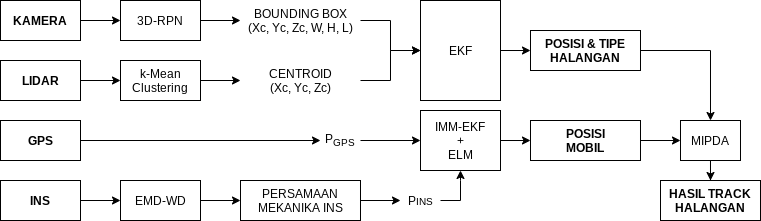
\includegraphics[width=\textwidth]{3-sistem.png}
    \end{center}
\end{frame}


\begin{frame}
    \frametitle{INS: Wavelet Denoising}
    EMD mendekomposisi sinyal x menjadi beberapa Instrinsic Mode Function (IMF). Hasil dekomposisi berbentuk jumlahan n komponen IMF dan sinyal residual. $c_n(t)$ merupakan komponen IMF, dan $r_n(t)$ merupakan sinyal residual
    \begin{equation}
        x(t)=\sum_{i=1}^{n} c_{i}(t)+r_{n}(t)
    \end{equation}
    Kemudian dilakukan wavelet denoising pada setiap komponen IMF, sehingga menghasilkan
    \begin{equation}
        x^{\prime}(t)=\sum_{i=1}^{n} c_{i}^{\prime}(t)+r_{n}^{\prime}(t)
        \label{eq: 4-PRE-denoised-x}
    \end{equation}
\end{frame}


\begin{frame}
    \frametitle{INS: Persamaan Mekanisasi}
    \begin{center}
        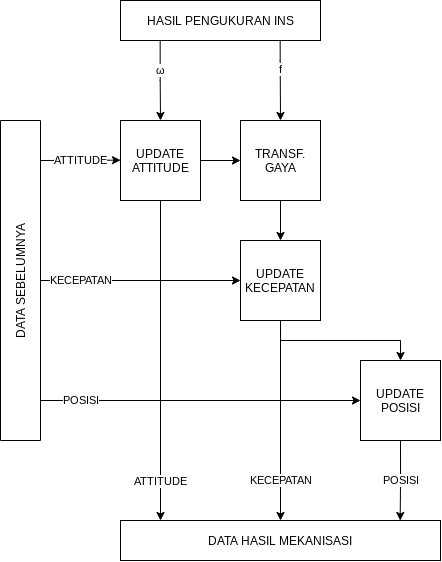
\includegraphics[width=.3\textwidth]{3-INS-mechanization.png}
    \end{center}
\end{frame}


\begin{frame}
    \frametitle{Model Data Lidar dan Kamera}
    Hasil kMeans pada deteksi Lidar berupa titik koordinat tiga dimensi dengan data berbentuk nilai centroid
    \begin{equation}
        w_{\text{lidar},i}^{t}=\left\{x_{\text{lidar}, i}^{t}, y_{\text{lidar}, i}^{t}, z_{\text{lidar},i}^{t}\right\}
    \end{equation}
    
    \vspace{2em}

    Hasil deteksi kamera berupa titik koordinat tiga dimensi dari centroid dan klasifikasi dari objek yang terdeteksi, yang tidak diproses menggunakan EKF, dan disimpan untuk penggunaan di penamaan track hasil MIPDA.
    \begin{equation}
        w_{\text{kamera},i}^{t}=\left\{x_{\text{kamera}, i}^{t}, y_{\text{kamera}, i}^{t}, z_{\text{kamera},i}^{t}\right\}
    \end{equation}
\end{frame}


\begin{frame}[allowframebreaks]
    \frametitle{Model State dan Pengukuran}
    \justifying
    $x_{j}^{t}, y_{j}^{t}, z_{j}^{t}$ merupakan posisi dari halangan relatif terhadap kendaraan, $V_{j}^{t}$ merupakan estimasi kecepatan halangan dan $\alpha_{j}^{t}$ merupakan estimasi yaw dari halangan. Vektor state $\varphi_{j}^{t}$ dapat dituliskan
    \begin{equation}
        \varphi_{j}^{t}=\left\{x_{j}^{t}, y_{j}^{t}, z_{j}^{t}, V_{j}^{t}, \alpha_{j}^{t}\right\}
    \end{equation}

    vektor pengukuran merupakan gabungan dari pengukuran posisi oleh lidar dan kamera.
    \begin{equation}
        w_{i}^{t}=\left\{x_{\text{lidar}, i}^{t}, y_{\text{lidar}, i}^{t}, z_{\text{lidar},i}^{t}, x_{\text{kamera}, i}^{t}, y_{\text{kamera}, i}^{t}, z_{\text{kamera},i}^{t}\right\}
    \end{equation}

    proses dari state dapat dituliskan
    \begin{equation}
        a_{j}^{t-1}=\left[\begin{array}{c}
        x_{j}^{t-1}+\Delta t V_{j}^{t-1} \cos \left(\alpha_{j}^{t-1}\right) \\
        x_{j}^{t-1}+\Delta t V_{j}^{t-1} \sin \left(\alpha_{j}^{t-1}\right) \\
        V_{j}^{t-1} \\
        \alpha_{j}^{t-1}
        \end{array}\right]
    \end{equation}

    matriks proses A dapat dicari dengan melakukan operasi jacobi pada $a_{j}^{t-1}$

    relasi antara vektor state dan pengukuran berbentuk persamaan nonlinier
    \begin{equation}
        w_{i}^{t}=\left[\begin{array}{c}
            x_{\text{lidar}, i}^{t}\\
            y_{\text{lidar}, i}^{t}\\
            z_{\text{lidar}, i}^{t}\\
            x_{\text{kamera}, i}^{t}\\
            y_{\text{kamera}, i}^{t}\\
            z_{\text{kamera}, i}^{t}\\
            \alpha_{i}^{t}
        \end{array}\right]^{T}=\left[\begin{array}{c}
        x_{j}^{t-1}+\Delta t V_{j}^{t-1} \cos \left(\alpha_{j}^{t-1}\right) +v_{x,j}\\
        y_{j}^{t-1}+\Delta t V_{j}^{t-1} \sin \left(\alpha_{j}^{t-1}\right)+v_{y,j}\\
        z_{j}^{t-1}+v_{z,j}\\
        x_{j}^{t-1}+\Delta t V_{j}^{t-1} \cos \left(\alpha_{j}^{t-1}\right)+v_{x,j}\\
        y_{j}^{t-1}+\Delta t V_{j}^{t-1} \sin \left(\alpha_{j}^{t-1}\right)+v_{y,j}\\
        z_{j}^{t-1}+v_{z,j}\\
        \alpha_{j}^{t-1}
        \end{array}\right]
    \end{equation} 

    dan nilai $H_j$ dapat dicari dengan menurunkan $w_{i}^{t}$
    \begin{equation}
        H_{j}^{t}=\frac{\partial h\left(w_{i}^{t}\right)}{\partial w_{i}^{t}}
    \end{equation}
\end{frame}


\begin{frame}
    \frametitle{Transformasi koordinat hasil deteksi}
    \justifying
    Sebelum masuk tahap tracking, posisi dari halangan akan ditransformasikan ke frame bumi menggunakan data posisi mobil. 
    
    Posisi kendaraan adalah vektor posisi $P = [p_x \quad p_y \quad p_z \quad \alpha \quad \beta \quad \gamma]'$, sementara itu posisi halangan adalah vektor posisi $S = [s_x \quad s_y \quad s_z]'$. Transformasi posisi halangan menjadi posisi absolut terhadap frame bumi dapat dilakukan menggunakan kombinasi matriks rotasi:

    \begin{equation}
        R(\alpha, \beta, \gamma)=
        \left(\begin{array}{ccc}
        c \alpha c \beta & c \alpha s \beta s \gamma-s \alpha c \gamma & c \alpha s \beta c \gamma+s \alpha s \gamma \\
        s \alpha c \beta & s \alpha s \beta s \gamma+c \alpha c \gamma & s \alpha s \beta c \gamma-c \alpha s \gamma \\
        -s \beta & c \beta s \gamma & c \beta c \gamma
        \end{array}\right)
    \end{equation}
    Sehingga posisi halangan terhadap frame bumi $T$ dapat dihitung dengan
    \begin{equation}
        T = R(\alpha, \beta, \gamma)S + [p_x \quad p_y \quad p_z]'
    \end{equation}
\end{frame}


\begin{frame}
    \frametitle{Hipotesa Penelitian}
    \justifying
    Dengan melakukan penggabungan beberapa sensor deteksi halangan (Lidar dan Kamera) dengan sensor deteksi posisi (INS dan GPS), diharapkan hasil tracking yang didapatkan lebih baik dibandingkan dengan tanpa melakukan penggabungan data.
\end{frame}


\begin{frame}
    \frametitle{Rencana Pengujian}
    \justifying
    Pengujian akan dilakukan untuk membuktikan hipotesa yang telah dibuat. Rencana pengujian yang akan dibuat terbagi menjadi tiga jenis pengujian:
    \begin{itemize}
        \item Pengujian hasil deteksi posisi halangan
        \item Pengujian posisi mobil
        \item Pengujian metode tracking
    \end{itemize}
\end{frame}


\begin{frame}
    \frametitle{Pengujian hasil deteksi posisi halangan}
    \justifying
    Pengujian ini dilakukan untuk menguji hasil sensor fusion kamera dengan lidar yang dihasilkan oleh EKF. Pengujian hasil deteksi posisi halangan ini akan dilakukan dengan beberapa variasi jarak dan jumlah halangan. Pada pengujian ini, akan dilakukan perbandingan metode sensor fusion pada tingkat fitur menggunakan SAF-FCOS dengan metode fusion pada tingkat data menggunakan EKF.
\end{frame}


\begin{frame}
    \frametitle{Pengujian posisi mobil}
    \justifying
    Pengujian ini dilakukan untuk menguji hasil sensor fusion dari GPS dan INS yang dihasilkan oleh IMM-EKF. Pengujian hasil deteksi posisi mobil otonom ini akan dilakukan dengan beberapa variasi lintasan, yakni:
    \begin{enumerate}
        \item lintasan lurus
        \item lintasan memutar
        \item lintasan berliku
    \end{enumerate}
\end{frame}


\begin{frame}
    \frametitle{Pengujian metode tracking}
    \justifying
    Pengujian ini dilakukan untuk menguji hasil tracking yang dihasilkan oleh metode Multi-Object Integrated Probabilistic Data Association. Pengujian hasil tracking ini akan dilakukan dengan beberapa variasi skenario, yakni:
            \begin{enumerate}
                \item tracking pada 1 objek
                \item tracking pada 2 objek
                \item skenario halangan 1 mendahului halangan 2.
                \item skenario halangan 1 berpapasan dengan halangan 2.
                \item skenario (1-4) dengan noise dan information loss pada hasil deteksi.
            \end{enumerate}
\end{frame}